
\section{Evaluation}

\eat{energy/graphs/dummy/g1_energy/energy-server.pdf
graphs/dummy/g1_energy/energy.pdf
graphs/dummy/g2_energy/energy.pdf
graphs/dummy/g3_availability/availability.pdf
graphs/dummy/g4_originrequests/origin.pdf
graphs/dummy/g5_onoff/onoff.pdf}

\begin{figure}[tbp]
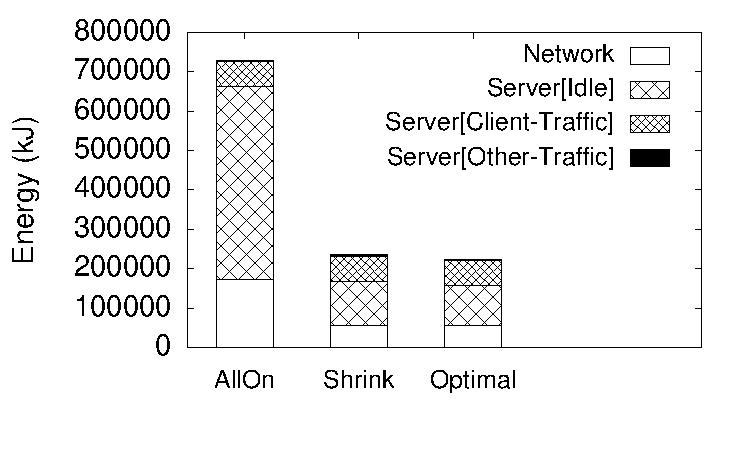
\includegraphics[scale=0.55]{energy/graphs/real/g1_energy/energy.pdf}
\caption{Datacenter energy use for an on-demand video workload for (1) AllOn scheme which keeps all servers and switches always on (2) \shrink\ (3) A lower-bound on energy consumption for this workload. \shrink\ reduces energy consumption by 67\% over AllOn scheme. Lower-bound on energy savings over AllOn scheme is 69\%.}
\end{figure}

\begin{figure}[tbp]
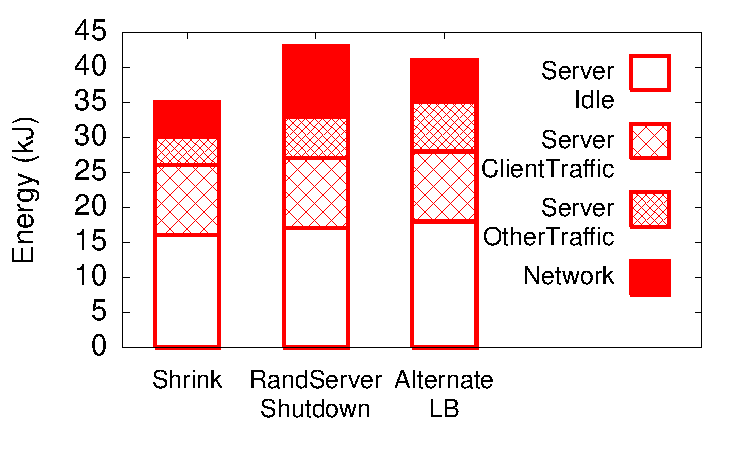
\includegraphics[scale=0.55]{energy/graphs/dummy/g2_energy/energy.pdf}
\caption{Comparison of other strategies for energy minimization.}
\end{figure}


\begin{figure}[tbp]
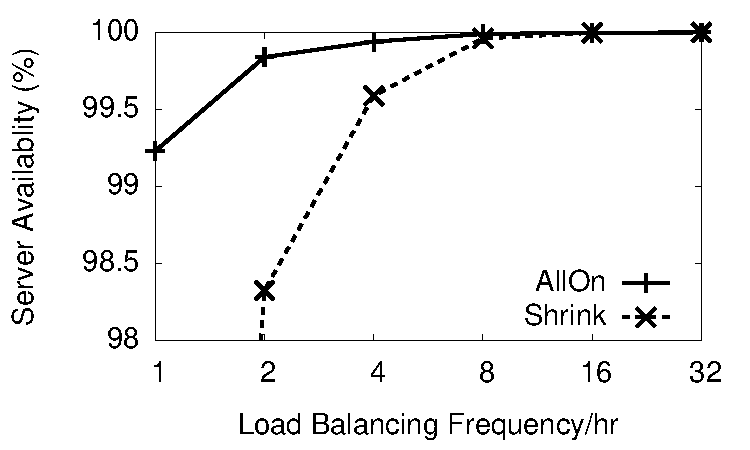
\includegraphics[scale=0.55]{energy/graphs/real/g3_availability/availability.pdf}
\caption{Fraction of requests that find the server available to serve the request. Both \shrink\ and AllOn achieve greater than than three nines availability when load balancing is done at a frequency of 32/hr ($\approx$ once every 2 min) or faster.}
\end{figure}


\begin{figure}[tbp]
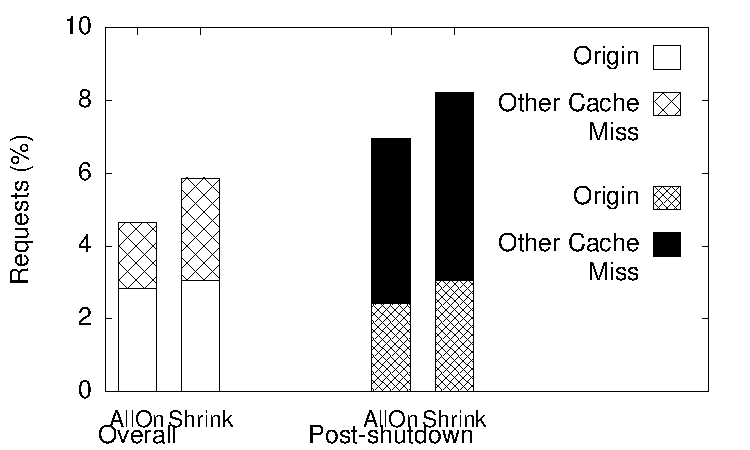
\includegraphics[scale=0.55]{energy/graphs/real/g4_originrequests/origin-2.pdf}
\caption{Comparison of requests served by origin overall. 2.82\% requests are served by origin servers with AllOn scheme, and 3.3\% requests are served by origin servers with \shrink.}
\end{figure}


\begin{figure}[tbp]
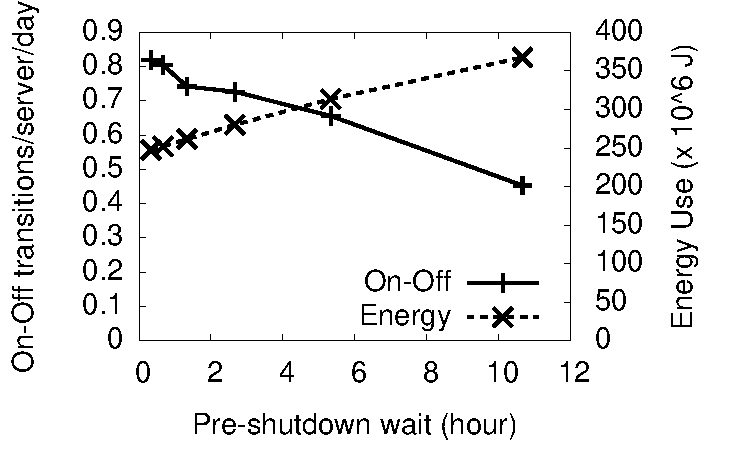
\includegraphics[scale=0.55]{energy/graphs/real/g5_onoff/onoff.pdf}
\caption{Rate of on-off transitions. A pre-shutdown wait of 20 minutes or more is sufficient to reduce the rate of on-off transitions to less than one/day/server.}
\end{figure}

\begin{figure}[tbp]
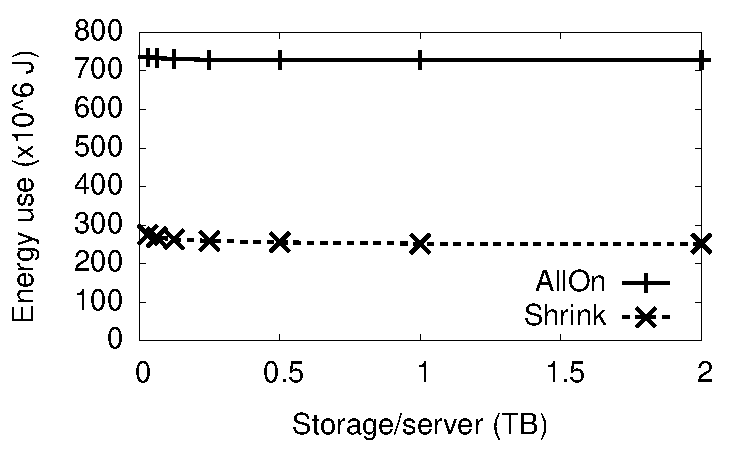
\includegraphics[scale=0.55]{energy/graphs/real/g6_storage/storage-energy.pdf}
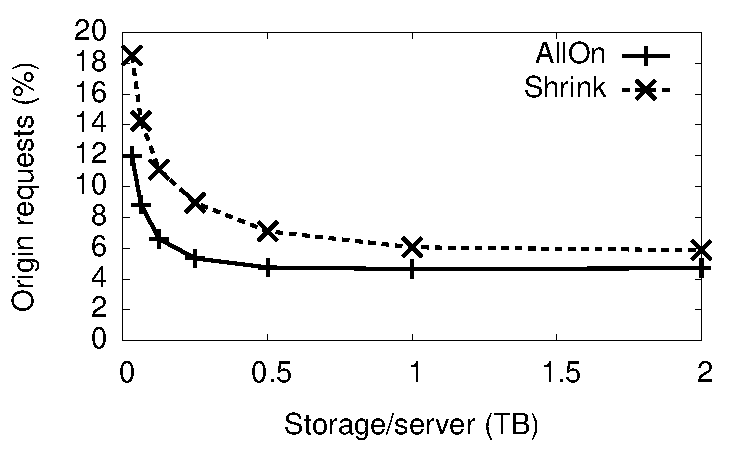
\includegraphics[scale=0.55]{energy/graphs/real/g6_storage/storage-missrate.pdf}
\caption{Energy use and fraction of requests sent to origin for varying storage/server. While energy use remains nearly equal for \shrink\ and AllOn schemes at all storage values, \shrink\ has a higher fraction of requests sent to origin when storage is lesser.}
\end{figure}
		


\begin{figure}[tbp]
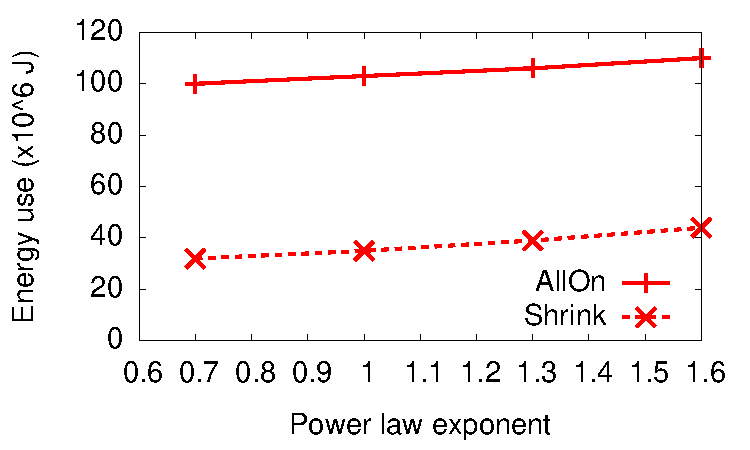
\includegraphics[scale=0.55]{energy/graphs/dummy/g7_popularity/popularity-energy.pdf}
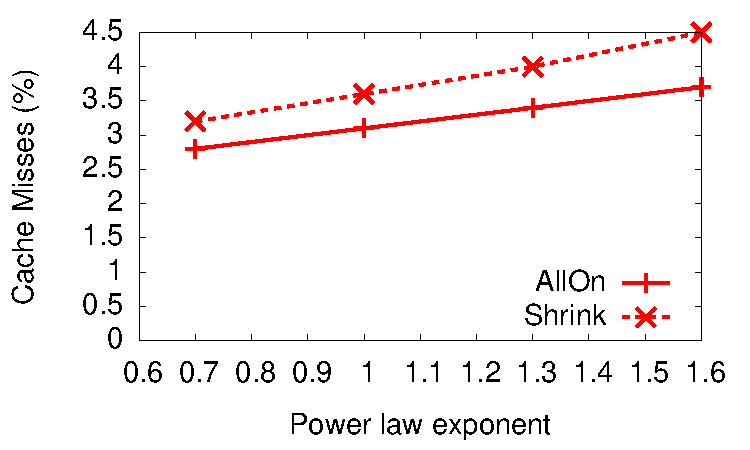
\includegraphics[scale=0.55]{energy/graphs/dummy/g7_popularity/popularity-missrate.pdf}
\caption{Energy use and cache hit rates for varying power-law popularity distribution of objects.}
\end{figure}

\begin{figure}[tbp]
\vspace{1.5in}
\caption{Experiments with downloads trace.}
\end{figure}



\begin{figure}[tbp]
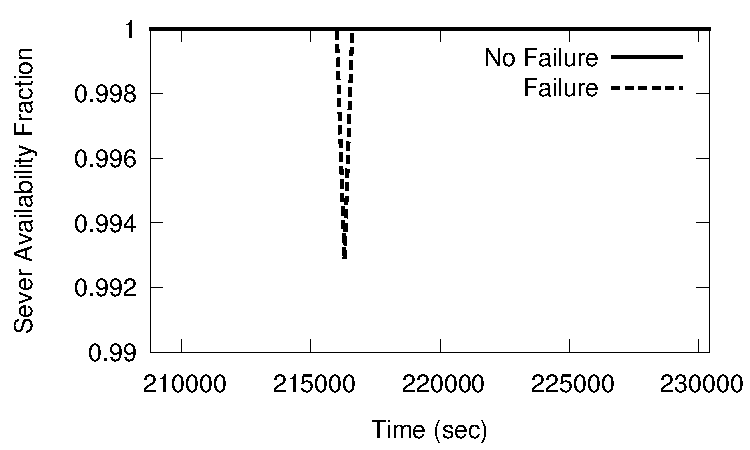
\includegraphics[scale=0.55]{energy/graphs/real/g8_serverfailure/cache-perf-denied.pdf}
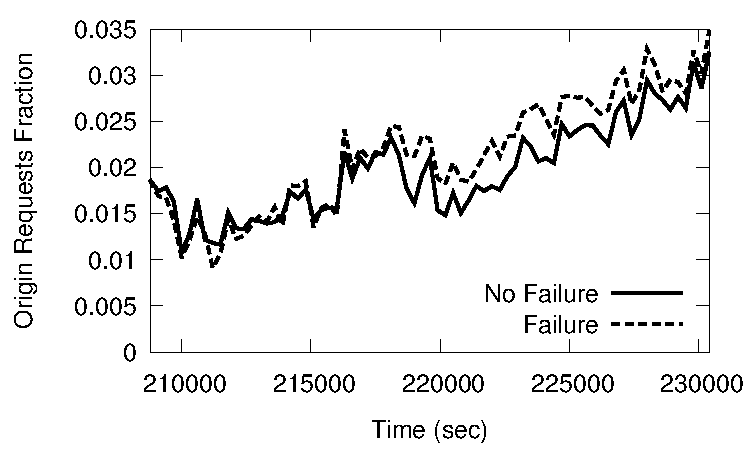
\includegraphics[scale=0.55]{energy/graphs/real/g8_serverfailure/cache-perf-origin.pdf}
\caption{Comparison of \shrink's performance in case of server failure vs a no-failure scenario. (Top) Immediately after a server failure, \shrink's availability drops to two-nines for until load-balancing is recomputed.  (Bottom) Fraction of requests sent to origin after a server failure and in a non-failure scenario are within 20\% of each other.}
\end{figure}

\begin{figure}[tbp]
\vspace{1.5in}
\caption{Experiment with switch failures.}
\end{figure}

\subsection{Experiments with \shrink\ protoype}


\subsection{Trace-driven experiments}




(1) Energy savings: AllOn, Shrink, LowerBound. (server part shows request \& content transfer energy).

Shrink, Shrink with random shutdown (error-bars),  Shrink with randomly shuffling load-balancing rules (error-bars).

(2) Availability: AllOn \& Shrink with different frequencies of adaptation; Shrink without considering initial utilization.

(3) OriginRequests: AllOn, Shrink (content-transfers), Shrink (pre-shutdown wait), Shrink (no effort).

(4) On-off transitions: Shrink with varying extra wait times for shutdown. Also show energy savings.


Other experiments:

(1) Storage: Origin requests. Fraction of energy savings.

(2) Traditional topologies: 

(3) Content chunking:  

(4) Fault tolerance: Server-fault tolerance, switch-fault tolerance.

%
%\begin{figure}
%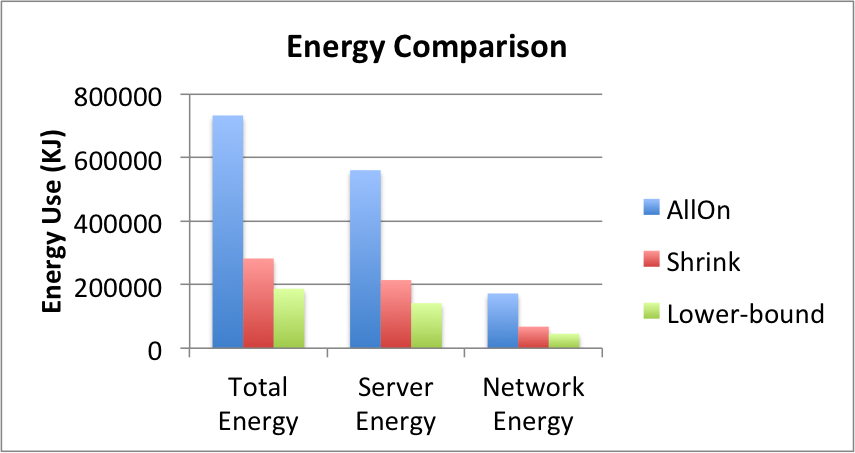
\includegraphics[scale=0.55]{energy/graphs/dec3/energy.png}
%\caption{Datacenter energy use for an on-demand video workload for (1) AllOn scheme which keeps all servers and switches always on (2) \shrink\ (3) A lower-bound on energy consumption for this workload. \shrink\ reduces energy consumption by 61\% over AllOn scheme. Lower-bound on energy savings over AllOn scheme is 74\%.}
%\end{figure}
%
%\begin{figure}
%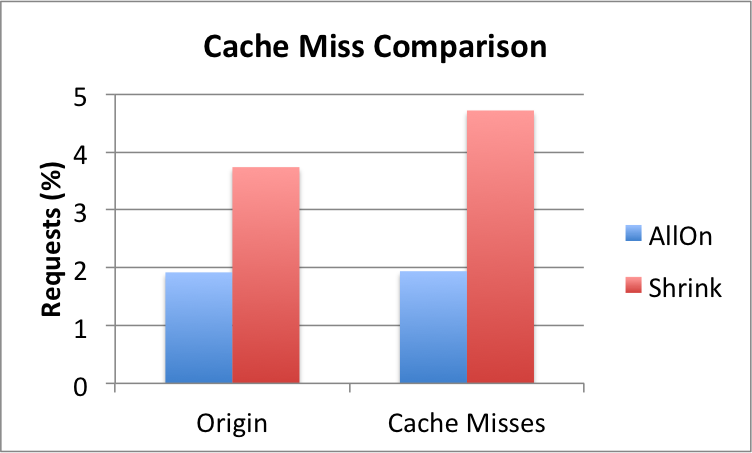
\includegraphics[scale=0.55]{energy/graphs/dec3/cachemiss.png}
%\caption{Comparison of cache misses: 1.92\% requests are served by origin servers with AllOn scheme, and 3.74\% requests are served by origin servers with \shrink.}
%\end{figure}
%
%\begin{figure}
%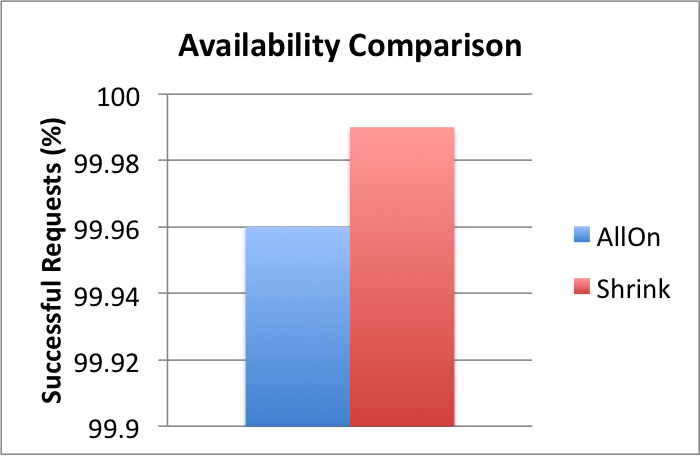
\includegraphics[scale=0.55]{energy/graphs/dec3/availability.png}
%\caption{Fraction of requests that find the server available to serve the request: \shrink\ and AllOn both have more than three nines availability of servers.}
%\end{figure}
%
